\begin{frame}{Recall}
    \begin{itemize}
        \item<1-> the input to a supervised learning algorithm is a training set ($x_{1:n}, y_{1:n}$), where
        \begin{itemize}
            \item<2-> $x_{1:n} = x_1,x_2,..., x_n$ shows input examples
            \item<3->  $y_{a:n}= y_1, y_2, ..., y_n$ shows corresponding labels
        \end{itemize}
        \item<4-> the goal of a learning algorithm is to return a function $f()$ that accurately maps input examples to their desired labels
        \uncover<5->{
        \begin{figure}
\centering
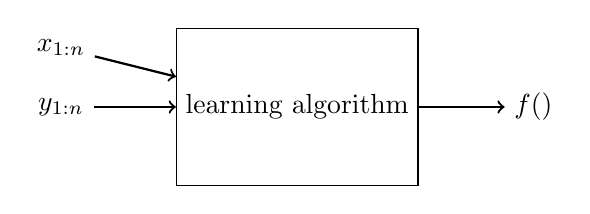
\begin{tikzpicture}

\node(x) at (0, 0) [] {$x_{1:n}$};
\node(y) at (0, -0.75) [] {$y_{1:n}$};


\node(lr) at (3,-0.75) [draw, minimum width=2cm, minimum height=2cm]{learning algorithm};

\draw[->,thick] (x) to (lr);
\draw[->,thick] (y) to (lr);

\node(f) at (6.0, -0.75) [] {$f()$};
\draw[->,thick] (lr) to (f);

\end{tikzpicture}
\end{figure}
        }
        \item<7-> the input to neural models $f()$ should be a numerical vector but NLP tasks are defined on texts
        \item<8-> how can we represent texts via numerical vectors? 
    \end{itemize}
\end{frame}
\begin{frame}{Text Representation \\ (a.k.a., Feature Extraction)}
    \begin{itemize}
        \item<1->  vector representation of a text should ideally reflect various linguistic properties of the text
        \item<2-> 
        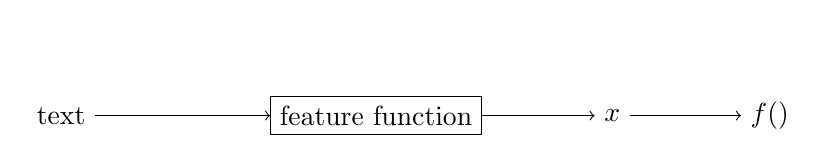
\begin{tikzpicture}
        \node[] () at (0,1) {};
        \node[] (text) at (0,0) {text};
        \node[draw] (feat_ext) at (4,0) {feature function};
        \node[] (x) at (7,0) {$x$};
        \node[] (f) at (9,0) {$f()$};
        
        
        \draw[->] (text) -- (feat_ext);
        \draw[->] (feat_ext) -- (x);
        \draw[->] (x) -- (f);
        \end{tikzpicture}  
        \item<3-> in this lecture we focus on  feature functions rather than learning algorithms
    \end{itemize}
\end{frame}

\begin{frame}{Some Terminologies}
    \begin{itemize}
        \item<1-> letters: smallest units in a language $\rightarrow$ a,b,c,...
        \item<2-> tokens and words: tokens are outputs of a tokenizer and words are meaning-bearing units
        \begin{itemize}
            \item note: in this course we use the terms ``word" and ``token" interchangeably 
        \end{itemize}
        \item<3-> lemma: the dictionary entry of the word $\rightarrow$ ``book" is the lemma of ``booking", ``booked", and ``books"
            \begin{itemize}
                \item how to obtain lemmas? use morphological analyzers 
                \item are available for many languages
                \item lemmatization may not work for any sequence of letters e.g., for mis-spelling
            \end{itemize}
            
        \item<4-> stems: a shorter version of a word defined based on some language-specific heuristic $\rightarrow$ ``pictur'' is the stem of ``pictures'', ``pictured'', and ``picture''
        \begin{itemize}
            \item the output of a stemmer need not be a valid word
        \end{itemize}
    \end{itemize}
\end{frame}
\begin{frame}{Some Terminologies}
    \begin{itemize}
        \item lexical resources: provide some information about words and their relations
        \begin{itemize}
            \item<1-> dictionaries
            \item<2-> WordNet for English
                \begin{itemize}
                    \item<3-> capture semantic knowledge about words
                    \item<4-> each word is associated with one or several synsets
                    \item<5-> synsets are linked to each other according to semantic relations  between their words
                    \item<6-> semantic relations are: hypernym (more specific),  hyponym (less specific), antonyms, holonyms (part-whole), and meronyms (whole-part) 
                    \item<7-> contains information about nouns, verbs, adjectives, and adverbs
                    \item<8-> manually created
                \end{itemize}
            \item<9-> FrameNet and VerbNet for English
            \begin{itemize}
                \item<10-> focus around verbs
                \item<11-> manually created
            \end{itemize}
            \item<12-> Paraphrase Database (PPDB) 
            \begin{itemize}
                \item<13-> contains paraphrases 
                \item<14-> automatically created
            \end{itemize}
        \end{itemize}
    \end{itemize}
\end{frame}
\begin{frame}{Common Features for Textual Data}
    what information can  we extract directly from  a word 
    \begin{itemize}
        \item<1-> letters comprising a word and their order
        \item<2-> length of word
        \item<3-> is the first letter capitalized?
        \item<4-> does word include hyphen? 

    \end{itemize}
    
\end{frame}
\begin{frame}{Common Features for Textual Data}
    \begin{itemize}
        \item<1-> Bag-of-Words (BoW): the count of each word in a text is taken as a feature
            \begin{figure}
                \centering
                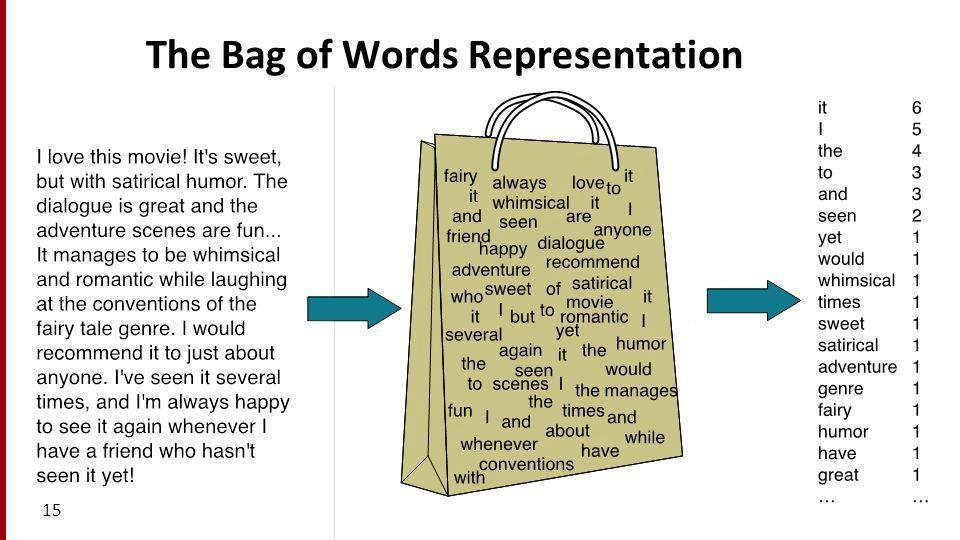
\includegraphics[scale=0.25]{./figure/bow.jpg}
            \end{figure}
    \item<2-> BOW does not care about the order of words
    \end{itemize}
    
    
    \vspace*{\fill}
     \textit{\tiny{(Taken from:\url{https://www.programmersought.com/article/4304366575/)}}}
\end{frame}
\begin{frame}{Common Features for Textual Data}
    \begin{itemize}
        \item<1-> TF-IDF: Term Frequency - Inverse Document Frequency
        \item<2-> let $d$ be a document from a given corpus $D$
        \item<3-> we map word $w$ of $d$ to a number as follows:
        
        \begin{equation*}
            \frac{\#(w,d)}{\sum_{w^\prime}  \#(w^\prime, d)} \times \text{log}\frac{|D|}{|\{ d\in D: w \in d\}|}
        \end{equation*}
        \item<4-> N-grams: instead of using the frequency of a word, we use the frequency of N sequence of words 
        \item<5-> N=2 $\rightarrow$ bi-gram 
        \item<6-> N=3 $\rightarrow$ tri-gram
    \end{itemize}
\end{frame}
\begin{frame}{Common Features for Textual Data}
\begin{itemize}
\item<1-> context: each piece of a text occurs within a larger text which is known as context
\item<2-> how to encode contextual information?
    \item<3-> using position of a word within a sentence or a document
    \item<4-> using the words that appear in an immediate context of a word
    \begin{itemize}
        \item<5-> immediate context: a window of $k$ words surrounding the target word
        \item<6-> ``the cat \underline{sat} on the mat'' , $k$=2 $\rightarrow$ $\{$ word-minus-2=the, word-minus-1=cat, word-plus-1=on, word-plus-2=the $\}$
    \end{itemize}
\end{itemize}
\end{frame}
\begin{frame}{Common Features for Textual Data}
    what information can we extract from the relation of text with external source of information?
    \begin{itemize}
        \item<1-> is a word in a list of common person names in Germany? 
        \item<2-> is a word a female or male person name?
        \item<3-> what is the lemma of the word?
        \item<4-> what is the stem of the word?
        \item<5-> what information do lexical resources give us about the word?
    \end{itemize}
\end{frame}
